\chapter{Case Analysis (Data and Evidence)}
\label{ch:analysis}

\section{Description of the data and evidence}

The case rests on two completed studies. The first is a set of component-level experiments on the implementation, run without a language model. The second is a seeded simulation that carries those measurements through the agent's control flow under stated assumptions. To keep the two apart, every number in this report belongs to one of six evidence classes (Table~\ref{tab:classes}).

\begin{table}[h]
\caption{Evidence classes used for every number in the report}
\label{tab:classes}
\small\singlespacing
\begin{tabularx}{\textwidth}{|p{2.6cm}|L|}
\hline\hrow \textbf{Class} & \textbf{Meaning}\\\hline
\textsc{actual} & Executed or measured on the implementation\\\hline
\textsc{synthetic} & Produced by the simulation; not a measurement of the agent\\\hline
\textsc{assumed} & An input value chosen by the authors\\\hline
\textsc{derived} & Computed from existing results\\\hline
\textsc{literature} & Taken from cited work\\\hline
\textsc{proposed} & Designed but not implemented, or not yet done\\\hline
\end{tabularx}
\end{table}

Table~\ref{tab:data} lists the data analysed. The gate study ran on 2026-10-04 in a Linux container (4-core Xeon at 2.1\,GHz, no GPU) with Python~3.11.15, Playwright~1.56.0, Chromium~141, LangGraph~1.2.12 and Chroma~1.5.9. The component latencies were measured on 2026-10-23 on a 2.8\,GHz container.

\begin{table}[h]
\caption{Data and evidence used in the analysis}
\label{tab:data}
\small\singlespacing
\begin{tabularx}{\textwidth}{|L|p{2.2cm}|L|}
\hline\hrow \textbf{Data set} & \textbf{Class} & \textbf{Size and content}\\\hline
Gate states: design, held-out 1, held-out 2 & \textsc{actual} & 38, 12 and 42 constructed states (goal, URL, served HTML, answer, oracle label)\\\hline
Ablation & \textsc{actual} & Each conjunct removed in turn on all 92 states\\\hline
Component latency & \textsc{actual} & 30 repetitions each of navigate, click, fill, DOM extraction, screenshot and $\Phi$ on self-hosted pages\\\hline
Recovery classification & \textsc{actual} & 6 failure messages through the real recovery engine\\\hline
Memory retrieval & \textsc{actual} (synthetic corpus) & 10 queries over 22 stored records\\\hline
Egress test & \textsc{actual} & 70 control-loop episodes, every socket connection logged\\\hline
Oracle validation & \textsc{actual} & 114 scripted trajectories\\\hline
Test suite & \textsc{actual} & 147 tests\\\hline
Simulation v2 & \textsc{synthetic} & 100 scenarios (seed 202), 1{,}000 Monte Carlo sets, sensitivity sweeps\\\hline
\end{tabularx}
\end{table}

\section{Method of analysis}

\subsection{The completion predicate}
The agent observes an environment state $s_t$ through an observation $\Omega(s_t)$: URL, title, element list and screenshot. A planner maps a goal $g$, a plan $P=(g_1,\dots,g_n)$ and the observation to an action $a_t$. Executing it returns a \emph{dispatch flag} $\alpha_t\in\{0,1\}$, which says only that the call returned without error. The agent may report completion only when a predicate holds on the state observed \emph{after} the action:
\begin{equation}
\Phi(g,s_{t+1},P,\sigma) = \bigwedge_{c\in C(g,P)} c(s_{t+1}) \;\wedge\; \pi(P) \;\wedge\; \neg\beta(s_{t+1},\sigma),
\label{eq:phi}
\end{equation}
where $C(g,P)$ is the set of postconditions implied by the goal and plan, $\pi(P)$ states that no plan step is pending, and $\beta$ is a blocking condition (a bot-check page, an unapproved high-risk action) with $\sigma$ the approval state. Dispatch does not imply completion: $\alpha_t=1\not\Rightarrow\Phi=1$.

In the implemented browser predicate, $\Phi$ is the conjunction of six checks (Table~\ref{tab:conj}), each instantiated only when its trigger words occur in the request, plus a pre-check for $\beta$ that halts the task as \textsc{Blocked}. Fig.~\ref{fig:verify} shows the decision path.

\begin{table}[h]
\caption{Conjuncts of the implemented completion predicate $\Phi$}
\label{tab:conj}
\small\singlespacing
\begin{tabularx}{\textwidth}{|p{0.8cm}|p{3.2cm}|L|}
\hline\hrow \textbf{Check} & \textbf{Name} & \textbf{Fails when}\\\hline
$E$ & Error state & Browser-error URL; error or ``not found'' title; bot-check URL or title; redirect to a sign-in page when the request named another URL\\\hline
$H$ & Search home & Still on a search engine's home page when a search, extraction or multi-step plan was requested\\\hline
$Q$ & Query & The results page does not carry the query quoted in the request\\\hline
$T$ & Typed text & The text the request asks to enter is not present in an input (exactly, if the request says ``exactly'')\\\hline
$X$ & Extraction & For extraction requests, no answer that mentions a content word of the request\\\hline
$R$ & Remaining steps & A multi-step plan still has a pending step and no structured extraction exists\\\hline
$\beta$ & Bot-check pre-check & A CAPTCHA or security-check page is detected; the task halts as \textsc{Blocked}\\\hline
\end{tabularx}
\end{table}

\begin{figure}[h]
\centering
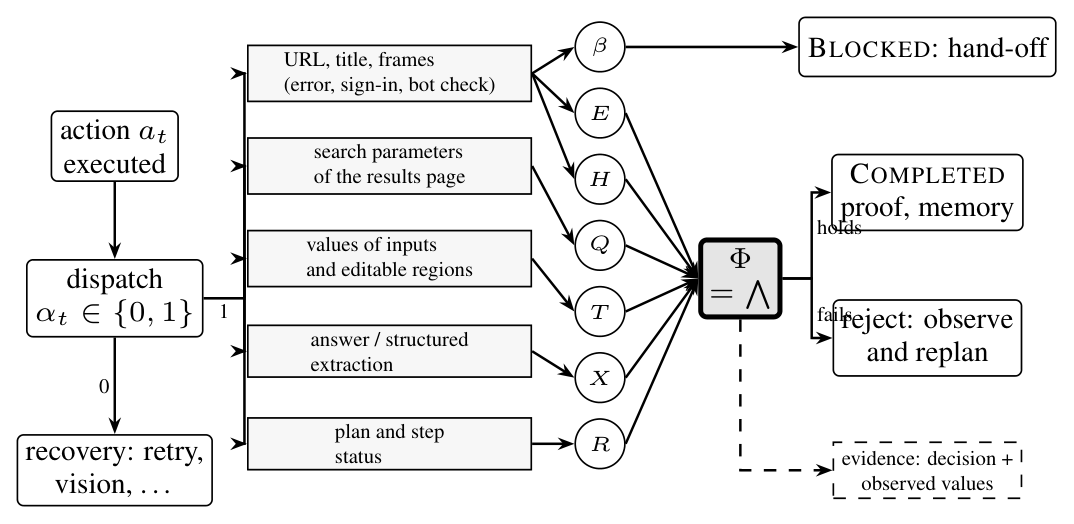
\includegraphics[width=0.9\textwidth]{fig/verification.png}
\caption{Decision path of the verification node: pre-check $\beta$, then the conjuncts of $\Phi$; only a passing state can end the task as \textsc{Completed}}
\label{fig:verify}
\end{figure}

\subsection{Metrics}
Let $\mathcal{T}$ be a set of end states, $\mathcal{T}_c$ those reported complete, and $\Phi^{\star}$ an oracle that shares no code with $\Phi$. With $N_{\mathrm{FC}}$ the states reported complete that the oracle marks unsatisfied, and $N_{\mathrm{FR}}$ the satisfied states not reported complete,
\begin{equation}
\mathrm{FCR} = \frac{N_{\mathrm{FC}}}{\lvert\mathcal{T}_c\rvert}, \qquad
\mathrm{FRR} = \frac{N_{\mathrm{FR}}}{\lvert\{\tau\in\mathcal{T}:\Phi^{\star}(\tau)=1\}\rvert}.
\label{eq:fcr}
\end{equation}
Because a dispatch-only rule reports every state complete, I also report the share of unsatisfied states that the gate withholds. Counts carry Wilson 95\% intervals~\cite{wilson1927probable}; paired comparisons on the same states use the exact McNemar test~\cite{mcnemar1947note} on decision correctness.

\subsection{Gate study design}
A state is a goal, a URL, an HTML document served through Playwright request interception, the agent's answer and plan state where relevant, and an oracle label. Every state ends with a dispatched action, so a dispatch-only rule accepts all of them. The \emph{design} set (38 states in six categories) was used to find the gate's defects and design fixes. \emph{Held-out~1} (12 states) was written after the fixes and not used to change them. \emph{Held-out~2} (42 states, 22 unsatisfied) was written to a fixed procedure with varied user phrasings and committed (\texttt{b9d5088}, SHA-256 recorded) before the gate was run on it. Each state is judged by the predicate called directly and by the real verification node with database, browser-pool and evidence I/O stubbed. Latency is the median of 20 repetitions after a warm-up.

\subsection{Simulation design}
The simulation draws 100 scenarios (seed 202), each with a task category and an outcome class that sets whether the goal is met. Detection and false-rejection rates are derived from the held-out gate states, latencies are resampled from the component measurements, and planner behaviour is assumed: chiefly the probability $\pi=0.65$ that a point at which the code evaluates $\Phi$ is reached while the task is unfinished, swept from 0.3 to 0.95. Monte Carlo replications regenerate 1{,}000 scenario sets with rates drawn from their Beta posteriors. The first model (v1) was committed before its scenarios were generated; an audit found four places where it contradicted the code, and the reported model, v2, was written after the v1 results were known. It is therefore post hoc, and the corrections moved results in favour of $\Phi$.

\section{Analysis and results}

\subsection{Completion gate (G1)}
Table~\ref{tab:gate} and Fig.~\ref{fig:gatechart} report the gate study (\textsc{actual}).

\begin{table}[h]
\caption{Completion gate on constructed states (\textsc{actual}). Withheld: unsatisfied states not reported complete. FR: satisfied states rejected. $p$: exact McNemar on paired correctness}
\label{tab:gate}
\small\singlespacing
\begin{tabularx}{\textwidth}{|L|c|c|c|c|}
\hline\hrow \textbf{Set and rule} & \textbf{Withheld} & \textbf{FR} & \textbf{$p$ vs dispatch-only} & \textbf{$p$ vs $E$ only}\\\hline
Design, before fixes (predicate) & 15/23 & 3/15 & -- & --\\\hline
Design, before fixes (live node, empty / verbose reasoning) & 14/23, 13/23 & -- & -- & --\\\hline
Design, after fixes$^{a}$ & 20/23 & 1/15 & -- & --\\\hline
Held-out 1 & 2/5 & 1/7 & 1.0 & 1.0\\\hline
Held-out 2 (frozen) & 9/22 & 1/20 & 0.021 & 0.070\\\hline
Pooled held-out & 11/27 & 2/27 & 0.022 & 0.11\\\hline
$E$ only, held-out 2 & 2/22 & 0/20 & -- & --\\\hline
Dispatch-only, any set & 0 & 0 & -- & --\\\hline
\end{tabularx}

\vspace{2pt}
\raggedright\footnotesize $^{a}$No test is reported on the design set, because the fixes were designed on it. Wilson 95\% intervals: design withheld 0.68--0.95; held-out 2 withheld 0.23--0.61, FR 0.01--0.24.
\end{table}

\begin{figure}[h]
\centering
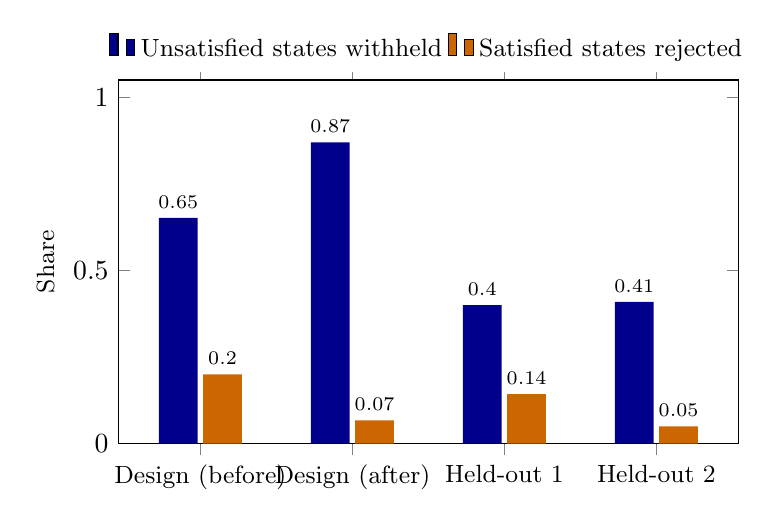
\begin{tikzpicture}
\begin{axis}[ybar, bar width=14pt, width=0.78\textwidth, height=6.2cm,
  ymin=0, ymax=1.05, ylabel={Share}, ylabel style={font=\small},
  symbolic x coords={Design (before),Design (after),Held-out 1,Held-out 2},
  xtick=data, x tick label style={font=\small},
  legend style={at={(0.5,1.02)},anchor=south,legend columns=2,font=\small,draw=none},
  nodes near coords, every node near coord/.append style={font=\scriptsize,/pgf/number format/fixed,/pgf/number format/precision=2},
  enlarge x limits=0.18]
\addplot[fill=blue!55!black,draw=none] coordinates {(Design (before),0.652) (Design (after),0.870) (Held-out 1,0.400) (Held-out 2,0.409)};
\addplot[fill=orange!80!black,draw=none] coordinates {(Design (before),0.200) (Design (after),0.067) (Held-out 1,0.143) (Held-out 2,0.050)};
\legend{Unsatisfied states withheld, Satisfied states rejected}
\end{axis}
\end{tikzpicture}
\caption{Share of unsatisfied states withheld and of satisfied states rejected by the gate on each set (\textsc{actual}; counts in Table~\ref{tab:gate})}
\label{fig:gatechart}
\end{figure}

On the code before the fixes, the pre-check and $\Phi$ withheld 15 of the 23 unsatisfied design states and rejected 3 of the 15 satisfied ones. Inside the live verification node they withheld only 14 or 13, because the node let a premature \texttt{complete} action mark a pending step done and took the planner's reasoning for an answer. After the fixes all three modes agree on every state of every set. On the design states the gate withholds 20 of 23 and rejects 1 of 15, correcting 7 states relative to the earlier gate without breaking any.

The held-out sets give a less optimistic estimate. On held-out~2, frozen before testing, the gate withholds 9 of 22 unsatisfied states (0.41) and rejects 1 of 20 satisfied ones (0.05). It is correct alone on 9 states and wrong alone on 1, so it is correct on significantly more held-out states than a dispatch-only rule (exact McNemar $p=0.021$; pooled with held-out~1, 11 against 2, $p=0.022$). Against the stronger baseline of a detector that applies only the error check $E$, which withholds 2 of 22 and rejects none, the gate is correct alone on 7 states and wrong alone on 1 ($p=0.070$; pooled $p=0.11$). On new phrasings, then, the evidence that the checks beyond $E$ add accuracy is suggestive but not significant.

The misses follow from the rules. The answer check $X$ fires only on words such as ``extract'', so requests phrased ``tell me'' or ``what year'' are not checked; when it fires it accepts any answer that repeats a goal term. None of the 5 unsatisfied extraction states in held-out~2 is withheld. Unparsed text-entry phrasings, unfamiliar error titles and an add-to-cart click that added nothing also pass. The one false rejection is a page that merely mentions reCAPTCHA. The answer to G1 is a qualified yes.

\subsection{Contribution of each conjunct (G2)}
Table~\ref{tab:abl} gives the ablation (\textsc{actual}). Removing one check at a time raises false completions on the design states, most for the error check $E$ (3 to 8) and the search-home check $H$ (3 to 7), but changes at most three held-out decisions, and removing $Q$ or $X$ changes none. These checks rarely fire on phrasings they were not written for, so the gate's coverage, more than the strength of any single check, limits it. With at most five discordant states, the smallest attainable $p$ is 0.063, so the ablation is descriptive.

\begin{table}[h]
\caption{Per-conjunct ablation on the design states (\textsc{actual}): false completions (of 23) and false rejections (of 15)}
\label{tab:abl}
\small\singlespacing
\begin{tabular}{|l|c|c|c|c|c|c|c|c|}
\hline\hrow \textbf{Configuration} & \textbf{Full} & \textbf{$-E$} & \textbf{$-H$} & \textbf{$-Q$} & \textbf{$-T$} & \textbf{$-X$} & \textbf{$-R$} & \textbf{$-\beta$}\\\hline
False completions & 3 & 8 & 7 & 4 & 6 & 6 & 4 & 5\\\hline
False rejections & 1 & 1 & 1 & 1 & 1 & 0 & 1 & 1\\\hline
\end{tabular}
\end{table}

\subsection{Overhead}
$\Phi$ makes no model call and no browser action; it reads the page through the browser protocol. Over the 83 decisions that evaluate $\Phi$, the median latency was 26.8\,ms (90th percentile 29.5\,ms, 95th 30.3\,ms, maximum 34.6\,ms), and decisions stopped by the pre-check took at most 13.4\,ms. Table~\ref{tab:lat} puts this beside the other browser operations, measured on self-hosted pages, where $\Phi$ alone took 5.2\,ms.

\begin{table}[h]
\caption{Component latencies on self-hosted pages, 30 repetitions each (\textsc{actual}, 2.8\,GHz container)}
\label{tab:lat}
\small\singlespacing
\begin{tabular}{|l|c|c|}
\hline\hrow \textbf{Operation} & \textbf{Median (ms)} & \textbf{95th percentile (ms)}\\\hline
Navigate & 17.1 & 24.9\\\hline
Click & 65.2 & 106.2\\\hline
Fill text & 12.5 & 17.4\\\hline
DOM extraction & 76.4 & 105.6\\\hline
Screenshot & 61.3 & 93.6\\\hline
Predicate $\Phi$ & 5.2 & 6.9\\\hline
\end{tabular}
\end{table}

\subsection{Locality (G3)}
I ran 70 agent episodes (10 development tasks under 7 configurations, six with memory) through the real control loop and Chromium against local sites, with a scripted stand-in for the Ollama API on 127.0.0.1. Every \texttt{socket.connect} and \texttt{connect\_ex} call in the harness's eight Python processes was logged. All 555 connection attempts went to the stand-in on 127.0.0.1, and every page request that Playwright reported named host 127.0.0.1. A rerun on the clean commit \texttt{7133301} (agent code identical to \texttt{bf0a8a5}) gave the same result. Memory retrieval returned records in 54 of the 60 memory-enabled episodes. The stand-in performs no inference, and UDP, DNS lookups, the Playwright driver, Chromium and the model server were not instrumented; the result covers the agent's Python processes.

In addition, the model client refuses any endpoint whose host is not a loopback address or a \texttt{localhost} name, before connecting, unless the user sets \texttt{PILOT\_ALLOW\_REMOTE\_MODEL=true} (Listing~\ref{lst:locality}). Unit tests confirm that a remote model address is refused and that Chroma telemetry is off.

\subsection{Memory and recovery}
Memory retrieval was measured on 10 queries over 22 stored records (a synthetic corpus), 9 of which had a relevant record: precision at 3 was 0.52, the largest value attainable on this corpus; recall at 3 was 1.00; and the mean reciprocal rank was 0.93. In 3 of 10 queries, however, the top-ranked record was irrelevant or retrieval failed, because retrieval has no relevance threshold.

The recovery engine classified 6 failure messages and assigned the strategy sequence shown in Table~\ref{tab:rec}. A missing confirmation, where the task ended without its goal being met, was classified as \emph{unknown} and given the generic sequence; the engine does not recognise it.

\begin{table}[h]
\caption{Recovery classification of six failure messages by the real recovery engine (\textsc{actual})}
\label{tab:rec}
\small\singlespacing
\begin{tabularx}{\textwidth}{|p{3.2cm}|p{3.2cm}|L|}
\hline\hrow \textbf{Failure mode} & \textbf{Classified as} & \textbf{Strategy by retry count 0--5 (then exhausted)}\\\hline
Navigation failure & transient & retry, retry, alt.\ selector $\times2$, vision fallback $\times2$\\\hline
Timeout & transient & retry, retry, alt.\ selector $\times2$, vision fallback $\times2$\\\hline
Missing element & element not found & retry, retry, alt.\ selector $\times2$, vision fallback $\times2$\\\hline
Invalid submission & verification failed & retry, retry, replan $\times4$\\\hline
Unexpected state & vision needed & vision fallback $\times6$\\\hline
Missing confirmation & unknown & retry, retry, alt.\ selector $\times2$, vision fallback $\times2$\\\hline
\end{tabularx}
\end{table}

\subsection{Oracle validity and tests}
The end-to-end oracle agreed with the intended verdict on all 114 scripted trajectories. The informative cases are 35 correct solutions (no false negative) and 34 near misses (no false positive); the rest are negative by construction. This bounds errors only on anticipated behaviours. Of the 147 tests in the suite, 144 pass; the 3 failures need live websites or a running model.

\subsection{Simulation results (H1--H5)}
Table~\ref{tab:sim} summarises the seeded simulation. All its values are \textsc{synthetic} (simulation v2, revised post hoc): they follow from measured component behaviour and \textsc{assumed} planner behaviour, depend on those assumptions, and are not measurements of the agent.

\begin{table}[h]
\caption{Simulation results (\textsc{synthetic}, v2, post hoc; conditional on \textsc{assumed} inputs)}
\label{tab:sim}
\small\singlespacing
\begin{tabularx}{\textwidth}{|p{1.1cm}|L|L|}
\hline\hrow \textbf{Hyp.} & \textbf{Quantity} & \textbf{Result}\\\hline
H1 & False completions in 100 scenarios & 19 with $\Phi$ vs 28 without verification; paired reduction 0.11 per scenario [0.05, 0.18]; direction fixed by construction\\\hline
H2 & Correct decisions on 74 claims & 52 with $\Phi$ vs 46 accept-all; discordant 9/3, $p=0.15$; $\Phi$ better at $p<0.05$ in 42\% of Monte Carlo sets; not supported\\\hline
-- & Tasks achieved and reported & 44 with $\Phi$ vs 46 without verification\\\hline
H3 & Repeated workflows succeeding (of 44) & 19 without memory, 19 with memory, 20 with a proposed relevance filter\\\hline
H4 & Recoverable failures recovered (of 93) & 51 inline retries only, 68 with the engine, 87 with proposed evidence-guided recovery (by assumption)\\\hline
H5 & Mean episode time & $+2.6\%$ with $\Phi$; $+14\%$ with a model self-check\\\hline
\end{tabularx}
\end{table}

Two of the three false rejections by $\Phi$ in the simulation come from scenarios with missing evidence, which $\Phi$ rejects at an \textsc{assumed} rate of 0.8, whereas the measured false-rejection rate is 0 of 24. Fig.~\ref{fig:sens} shows the sensitivity to the unmeasured premature-claim rate $\pi$: the false completion rate is 0.14 with $\Phi$ against 0.21 without verification at $\pi=0.3$, and 0.32 against 0.45 at $\pi=0.95$, while the false rejection rate stays near 0.14 against 0.08.

\begin{figure}[h]
\centering
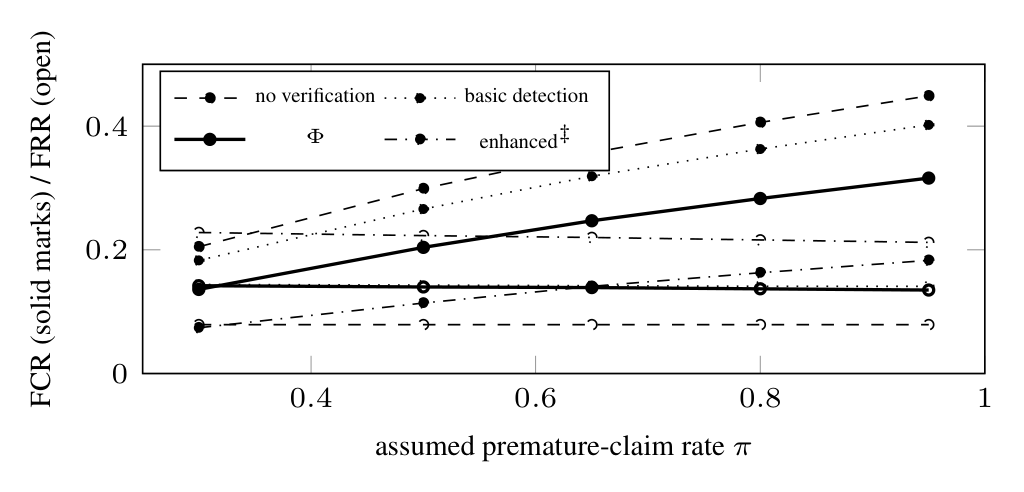
\includegraphics[width=0.72\textwidth]{fig/sensitivity.png}
\caption{Sensitivity of false completion and false rejection rates to the premature-claim rate $\pi$ (\textsc{synthetic}; 300 scenario sets per point)}
\label{fig:sens}
\end{figure}

\section{Validation of findings}

The findings were checked in four ways.
\begin{enumerate}
\item \textbf{Independent recomputation.} About 120 printed quantities were recomputed from the raw files with code that imported nothing from the project's analysis scripts. No numerical mismatch was found.
\item \textbf{Reproducibility.} The simulation, the table generators, the statistics script and the document build were rerun in fresh clones; all outputs were byte-identical.
\item \textbf{Freezing.} Held-out~2 was committed with its SHA-256 hash before the gate was run on it, and the code it ran on added only default-off switches and logging to the frozen gate.
\item \textbf{Agreement across modes.} After the fixes, the predicate called directly and the live verification node with empty or verbose reasoning agreed on every state.
\end{enumerate}

\section{Limitations of the data}

\begin{itemize}
\item The gate states are constructed, not sampled from real use. The states and their oracle labels were written by the AI assistant that also designed the gate fixes, and no second person relabelled them, so no inter-annotator agreement exists.
\item The sets are small. With 22 unsatisfied held-out states, the interval on the withheld share runs from 0.23 to 0.61.
\item The design-set result (20 of 23) is optimistic, because the fixes were made on those states.
\item The egress test used a scripted stand-in model server and logged only the Python processes' TCP connections.
\item Memory retrieval was measured on a small synthetic corpus with loosely grouped relevance labels.
\item The simulation is post hoc and conditional on assumed planner behaviour, above all the premature-claim rate $\pi$.
\item Task-level success of the full agent with a language-model planner was not measured in this study. A harness for it is released (Section~\ref{sec:harness}).
\end{itemize}
